\documentclass[conference]{IEEEtran}

\renewcommand\IEEEkeywordsname{Keywords}
\usepackage{biblatex}
\usepackage{graphicx}
\usepackage{mathtools}
\usepackage{enumitem}


\DeclarePairedDelimiter\floor{\lfloor}{\rfloor}


\begin{document}

\title{Identification of Anamalous Users in Twitter based on User Behaviour using Artificial Neural Networks}

\author{
\IEEEauthorblockN{Kiran K, C Manjunatha, P Deepa Shenoy, Venugopal K R}	
\IEEEauthorblockA{
Department of Computer Science and Engineering\\
University Visvesvaraya College of Engineering\\
Bangalore Karnataka\\
E-mail:manjunathagee@gmail.com
E-mail:kirank.uvce@bub.ernet.in
}

}

\maketitle

\begin{abstract}

Increased number of users in Online Social Networking(OSN) such as Facebook, Twitter, Instagram etc has led to privacy and security concerns. In this paper we proposed a behavioral based risk assessment method which will help to identity Social Bots and Compromised Accounts in Twitter by leveraging the Neural Networks.
Our solution can detect unusual accounts based on the users' writing style, such as, time of tweeting, language used for writing tweet, frequency of tweeting, etc. This way, if the writing style of the user changes 
from what is considered to be normal, we flag the user as risky and the OSN admin can formulate strategies to overcome the same. Experiments were performed 
on the real world dataset extracted from twitter. Results show tremendous accuracy in identifying Social Bots and that only few tweets are required to identify whether an account has been compromised or not.

\end{abstract}

\begin{IEEEkeywords}

Anamoly Detection, Compromised Account Detection, Neural Networks, Social Bots, Twitter.

\end{IEEEkeywords}

\section{Introduction}

Online Social Network (OSN) is a communication media where people share their thoughts, emotions and opinion about any subject. At present, Social networks like Facebook, Twitter, Instagram etc. are exposed
into area of information and research like Customer Relationship Management (CRM) and Opinion Mining (OM). Information extracted from Social Networks like Twitter and Facebook are extremely valuable for text mining, public opinion organisations, research and marketing companies.
In Social Networks, millions of opinions are expressed with simplicity, unbiased and easy content comprehension. hence dataset of Online Social Networks are valuable for decision making on 
business intelligence, marketing research,  image monitoring, and stock market prediction.

The wide popularity of Online Social Networks such as Facebook, Twitter, Instagram etc. and their ease of use have resulted in the compromise of their privacy and security of the users. 

Twitter is a microblogging and social networking  platform which enables registered users to read, write, retweet and reply etc. to other users with messages, so-called tweets.
According to a research \footnote{https://www.statista.com/statistics/282087/number-of-monthly-active-twitter-users/} the worldwide population of monthly active users is 336 million for the first quarter of 2018 and the number keeps increasing. A new study\footnote{https://www.cnbc.com/2017/03/10/nearly-48-million-twitter-accounts-could-be-bots-says-study.html} suggests 
that nearly 48 million twitter accounts are social bots, the accounts controlled by the software will generate the content algorithmically to influence the group and target specific category of accounts in social networks.

Many social bots perform many useful automated tasks such as creating scheduled news posts, weather updates etc. However, there is an incrased number of social bots which are created to perform malicious activites such as to support political agenda, promote terrorist activities for recuritment, to propogate fasle rumors and conspiracy theories. 

\section{Data Extraction}

Our data extraction process focused on extracting real world data with the help of a pyhton library called 'tweepy'. It starts with a given single user, extracts his/her friends then their friends in a recursive fashion till the count reaches a depth of 100, and for each user will extract features like user id, tweet id, time of tweet, langulage used for sending tweet, source, friends count, followers count, favorite count, user longevity.

For instance, for a user A is given, will extract 100 friends from the user profile, so the total number of users are 101, and for each of this 101 users we extract all the features from there public profile. We repeated this process of extraction for a period of 3 months starting from Feb 2018 at random time intervals. Care was taken to avoid repetative data extraction i.e if the data was already extracted for a user we skipped the data extraction for the next interval.

\section{Types of Attacks in OSN}
Attackers use OSN to propogate false agenda, extract personal information and even convince the users to provide sensitive financial data like credit card details, etc. They also convence users to click on a malicious links which will propagate the malicous contents on users wall. Below we take a look at well known types of attacks which happen in majority of OSNs.

\subsection{Sybil Attack}
Sybil attack is the most common type of attack in majority of the OSNs. In order to launch sybils, a malicious user has to create multiple fake accounts in order to gain his identity by targeting a particular community and starts sending friend requests. Once friend requests are accepted, over a period of time the attacker will convince the users to buy fake online products, provide credit card details, bank details and even convince the users to propagate the malicious links onto their walls.

\subsection{Cross-Site Scripting}
Compromised accounts are the accounts of real users who have lost their account credentials partially or completely. Attackers use cross-site scripting to steal user credentials by manipulating the login forms and Document Object Model(DOM). Once the attacker gets hold of the original credentials, user's friends are targeted to promote malicious contents very easily. Compromised account detection is not simple since the user is having legitimate relationship with his/her friends and followers over a period of time. Howerver, by monitering user's writing style over a period of time and by comparing with the new contents, compromised accounts can be detected.

\subsection{Socware Attacks}
Socware is derived from two words \textbf{soc}ial mal\textbf{ware}. Here, attackers create malicious links to lure people to click on it, acquire user credentials and spread malicious links on the user's wall or to support a particular false agenda. Upon clicking the link, attackers take users to some inappropriate sites or can even run the virus on user's machine to steal sensitive information.

\subsection{Creepers Attacks}
Creepers are real users who use OSN in inappropriate ways. For instance, they sometimes sell their account temporarily to some third party to promote advitisements or to promote some false agenda. By observing the types of links the user posts over a period of time and by analysing them against blocklisted urls, creepers accounts can be identified.

\subsection{Identity Cloning}
Identity cloning happens when an attacker makes an exact replica of an existing user account by collecting his/her public profile details and starts sending requests to their friends on their timeline. Once the requests are accepted, the attacker convinces the users to buy online fake product, post fake malicious links on their wall etc. over a period of time. By comparing the public profile amongst the close friends' circle identiy cloning can be identified.

\subsection{Cyber Bullying}
This is the common type of attack in OSN where an attacker repeatedly sends hurtfull messages, shares private pictures or videos of the victims(usually teenagers and children) and harass them. One way to identify this type of attack is to monitor the user's messages. If there are more incoming messages without any likes/shares/replies then there is a high probablity that the receiver is a victim of the attack.

\section{Releated Work}
Many approaches have been proposed by authors over a period of time in order to detect aforementioned types of attacks; SVM(Support Vector Machine) classifiers are used to seggregate the user's posts based on spam keyword score to identify the SocWare attack \cite{1}, Sybil detector apps were developed for RenRen(Chinese OSN) using regression by segregating the sybil accounts with the normal accounts based on user behaviour \cite{2} \cite{3}. COMPA app generated for facebook compares every message generated with the history of messages to flag compromised accounts, FRAppE generated for facebook successfully identifies the malicious apps by analysing the permissions which the apps requires during authentiction. \cite{4}.

Many of the previously proposed works on detecting bots are achieved by gaining the full access to all data. Wang at el proposed a method to cluster these collected data on the behavioral patterns of the users. Beutel et al. have broken down the event data in time, user, and activity dimensions to extract similar behaviors. These methods can be used to identify the large-scale attacks on twitter, directed at a common set of targets at the same time. But, the problem arrives when accounts with similar planning of attacks will target the different groups and can handle the account separately from each other.

One of the studies on detecting the spam twitter was done by the author Yardi et al. \cite{5} in the year 2010. They proposed a behavioral pattern to detect the accounts which are purely created to send the spam. But, they were able to find only small amount of differences when compared with the normal one. Social networks like Twitter will also react to the malicious spam problem by constantly trying to optimise its solutions to reduce the spammers. Another work done by Thomas et al. \cite{6} proposed a method to analyse the accounts blocked by the Twitter and they were able to find out that 77 percent of the spam accounts can be detected by the Twitter if blocked within 24 hours and 92 percent of the spam accounts within three days. However, many of the celebrities control more than hundred Twitter accounts and create new accounts to replace the blocked account.

Much of the research was done on spam on Twitter over many of the years. N.N. Patil, and N.S. Gawale proposed a system to detect URLs on Twitter which contain malicious content\cite{7}. One more method was proposed by the author Chen et al. \cite{8} which will assess the ability of malicious spam detection by using different machine learning algorithms. They found that Naive Bayes and SVM tend to outperform other classifiers on spam detection.

However, some of the accounts are lot harder to prevent which are not created for sending malicious content in the twitter. Less research is done on these compromised accounts. One of the methodology proposed by authors, G. Specht and  E.Zangerle, to find classified tweets which are being hacked is based on the behavioural reaction of the original user \cite{8}. Thomas et al. \cite{9} show the impact of the compromised account by uncovering the threat of cyber bullying, account hijacking and the damages they cause on the victim. The research done by Egele et al. \cite{10}  has the same approach as this study, wherein the authors propose a tool that identifies the compromised accounts on social network like Facebook and Twitter. The authors considered 6 feature to identify the compromised account in Facebook and Twitter, which are determined by the labelled training dataset of Facebook and Twitter, where each feature has its own weightage.

\section{Feature Extraction}
\label{featureDescription}
In this section we discuss the derived features which are used to train the Artifical Neural Network(ANN).

\subsection{FriendShip Ratio}
The normal behaviour of any user in any OSN is that, when he/she creates a new account the rate at which he/she makes friends is limited. By considering the rate at which an user sends a friend request, we can easily identify whether the account is a bot or not. The research done by Zhi Yang and Christo Wilson clearly shows that the bots are aggressive in establishing new connections with strangers in a small span of time. It can be noted that, if an user successfully establishes large number of connections within a short span of time, then it is not a normal behaviour \cite{11}.

\begin{equation}
	 FR (U) = \frac{|Friends(U)|}{User Longevity} \\
\end{equation}

Where \verb |Friends(U)| represents the total number of friends an user(U) has acquired and User Longevity is the total number of days since the user created the account in Twitter. 

\subsection{Tweet Ratio}
Similar to FriendShip Ratio we also compute the Tweet Ratio which indicates the frequency with which the user is sending tweets in OSN.
	
\begin{equation}
	 TR (U) = \frac{|Tweets(U)|}{User Longevity} \\
\end{equation}	

Where the \verb |Tweets(U)| is the total number of Tweets the user has sent and User Longevity is the total number of days since the user created the account in Twitter.

\subsection{Favorite Ratio}
Favorite Ratio signifies the rate at which the user likes other users posts in a short duration of time. 

\begin{equation}
	FAVR (U) = \frac{|Favorites(U)|}{User Longevity} \\
\end{equation}

Where the \verb |Favorites(U)| is the total number of likes the user has given and User Longevity is the total number of days since the user created the account in Twitter.

\subsection{Tweeting Period}
Here, we consider the time in which the user prefers to send the tweet during the 24 hours of the day. We divide the day into 4 quadrants and identify the quadrants in which the user prefers to send the tweet. If there is a sudden change in the tweeting period we assume that this is not a normal behaviour. \\

The algorithm to count the number of tweets by a user in the tweeting period is given in algorithm 1.

\textbf{Algorithm 1:} Creating Tweeting Period and counting number of tweets for each user in the Dataset DT; \\
\textbf{Input:} Preprocessed dataset DT; i=1,2,3...N, t=1,2,3,...M, contains the tweet creation time for each tweet t which belongs to user i;\\
\textbf{Output:} User time preference, duration of the day in which the user usually sends the tweet; \\

\begin{enumerate}
\item Iterate: \textit{i = 1} to \textit{N;}\\
Initialize quadrants for each user;\\
Q1 $\leftarrow$ 0; \\
Q2 $\leftarrow$ 0; \\
Q3 $\leftarrow$ 0; \\
Q4 $\leftarrow$ 0; \\
  \item Iterate: \textit{t=1} to \textit{M};
	\begin{equation*}
		\verb sent_time =  tweets[i][t].creation_time;
	\end{equation*}
	\begin{equation*}
		if( \floor*{\frac{sent_time}{6}}  == 0) ;
			Q1 \leftarrow Q1+1
	\end{equation*}
	\begin{equation*}
		else if( \floor*{\frac{sent_time}{6}}  == 1) ;
			Q2 \leftarrow Q2+1
	\end{equation*}
	\begin{equation*}
		else if( \floor*{\frac{sent_time}{6}}  == 2) ;
			Q3 \leftarrow Q3+1
	\end{equation*}
	\begin{equation*}
		else if( \floor*{\frac{sent_time}{6}}  == 3) ;
			Q4 \leftarrow Q4+1
	\end{equation*}
\end{enumerate}
\begin{equation*}
twitter[i][\verb tweeting_period] \leftarrow max(Q1, Q2 , Q3 , Q4)
\end{equation*}

\subsection{Device Preference}
Here, we track the device category that the user is using to compose tweets. Majority of the users tend to use the same category of devices like mobile phones, desktops, tablets etc. By tracking the device preference of an user we will be able to detect anamalous behaviour as shown in algorithm 2.

\textbf{Algorithm 2:} Computing the Device preference for each user in Dataset DT; \\
\textbf{Input:} Preprocessed dataset DT; i=1,2,3..N, t=1,2,3...M, contains the devices(t) used by user(i) for composing tweet;\\
\textbf{Output:} User device preference, common category of devices used to compose tweet; \\

\begin{enumerate}
	\item Iterate: \textit{i = 1} to \textit{N}; \\
	Initialize device preference  for each user \textit{i};
	\begin{equation*}
		\verb device_preference[i]  \leftarrow "";
	\end{equation*}
	\item Iterate: \textit{t = 1} to \textit{M};
		\begin{equation*}
			sources  \leftarrow \\availableSourceForUser[i]; \\
		\end{equation*}
		\begin{equation*}
			devicePreference[i]  \leftarrow
		\end{equation*}	
		\begin{equation*}
			numeric( asCharacter( max( sources )))
		\end{equation*}	
		
		
\end{enumerate} 
First, we extract all the devices that the user has used to compose the tweet, and in the next step we consider the most used device among the available sources. Since the ANN cannot work on the string sources, we convert the string sources to numeric values.

\subsection{Language Preference}
Here, we track the language that the user is using to compose tweets. Majority of the users tend to use the same language for composing the tweet. 
By tracking the language preference of an user we will be able to detect anamalous behaviour as shown in algorithm 3.

\textbf{Algorithm 3:} Computing the Language preference for each user in Dataset DT; \\
\textbf{Input:} Preprocessed dataset DT; i=1,2,3..N, l=1,2,3...M, contains the languages(l) used by user(i) for composing tweet;\\
\textbf{Output:} User language preference, common language used to compose tweet; \\

\begin{enumerate}
	\item Iterate: \textit{i = 1} to \textit{N}; \\
	Initialize language preference  for each user \textit{i};
	\begin{equation*}
		\verb language_preference[i]  \leftarrow "";
	\end{equation*}
	\item Iterate: \textit{l = 1} to \textit{M};
		\begin{equation*}
			sources  \leftarrow \\availableLanguagesForUser[i]; \\
		\end{equation*}
		\begin{equation*}
			languagePreference[i]  \leftarrow
		\end{equation*}	
		\begin{equation*}
			numeric( asCharacter( max( language )))
		\end{equation*}	
		
		
\end{enumerate} 
First, we extract all the languages that the user has used to compose the tweet, 
and in the next step we consider the most used language among the available languages. 
Since the ANN cannot work on the string sources, we convert the string sources to numeric values.


\section{Methodology}


Table 1 maps the well known OSN attacks i.e SocWare and Compromised Account to behavioural features\cite{11}. 
We use Friendship Ratio, Favorite Ratio and Tweet Ratio to identify wheather an account is SocWare or not, similarly we use Tweeting Period, 
Device Preference and Language Preference to identify wheather the account is compromised or not.

\begin{figure}[h!]
	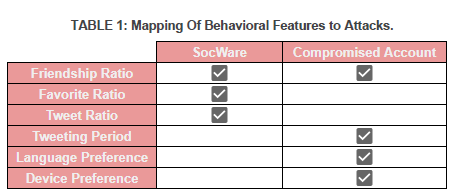
\includegraphics[scale=0.7]{attack_types1}
\end{figure}

The entire flow of anomalous user detection can be summerized as shown in Fig 1. The first step includes extraction of real world data. 
We have used python library called 'tweepy' for extracting the data in csv format.

The quality of the ANN algorithm depends directly on the quality of input data. Real world data tends to be messy with many missing values, 
redundant and noisy data etc. Hence, in the second step we carry out exploratory data analysis where we clean the data looking for missing, 
NotAvailable(NA) or empty values, duplicate ids and identify any outliers. Then we remove such data since they can make the ANN model unstable for prediction.

\begin{figure}[h!]
	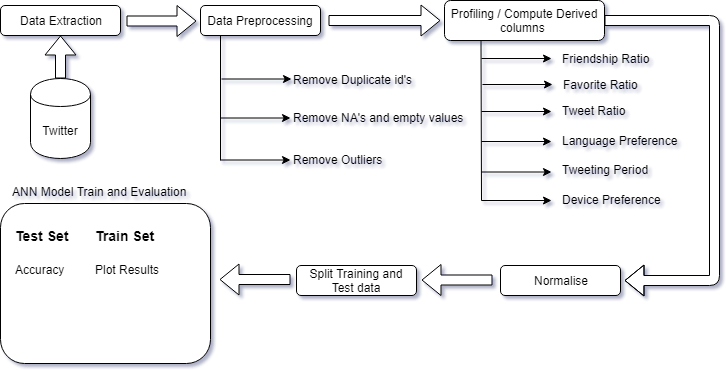
\includegraphics[scale=0.7]{Methodology}
	\caption{Flowchart of Anomalous User Detection.}
\end{figure}

In the third step we derive the columns like Friendship Ratio, Tweet Ratio, Tweeting Period, Device Preference using the algorithm discussed in section 
\ref{featureDescription}. The derived values are then normalized to scale within 0 to 1.

Once the data is preprocessed and all the derived columns are available, we split the data into train and test data, use the train data to prepare the ANN model and once the model is trained we use the remaining test data to evaluate the 
accuracy of the model to test how well the model has learnt from it's test data.

\section{Experiments and Results}
	  We considered extracting the real world data using python library called 'tweepy'. We started with one user and extracted all the friends 
	  from the user profile and extracted all the tweets and other information required for the algorithm and we repeated the same procedure for each 
	  of the friends in the list, taking care to avoid duplicated extraction of the user data who is a common friend. 
	   
	  Once the data is available, we carried out Exploratory Data Analysis to identify null/empty values and removed outliers from the data. 
	  Using the algorithms discussed in section \ref{featureDescription} we divided the data into training and test data in the ratio of 70:30(train:test).

	  We used Aritifical Neural Network library called 'neuralnet' provided by 'R' language. 
	  Once the model was trained we used the remainig test data to evaluate the performace of the ANN model, 
	  and once we noticed deviation in the user behaviour we flaged the user as anamalous.
	
	  While extracting the data we collected data samples of compromised account from twitter.com to see 
	  whether our algorithm is able to classify them as compromised or not. 
	  
	  We ran the algorithm on the 1.4 million tweets extracted from twitter, and were able to identify Social Bot accounts 
	  with high accuracy requiring only few tweets to identify whether the account is compromised or not.
	 
	  The final results classified those compromised accounts showing the accuracy of algorithm used.
	  
	  Authors\cite{12} used features like links and retweets for profiling the algorithm and N-grams as its kernal to classify the compromised account. They 
	  achieved results with accuracy ranging from 94.10\% to 95.80\%. We proposed a behavioural based methodology using features like friendShip ratio, favorite
	  ratio, tweet ratio, language preference, device preference, tweeting period to identify compromised account with an error rate of only 0.79\%.
 
 Fig 2. shows the sample of ANN as created by R neuralnet library. We used features like tweeting period, devices used for composing tweets, 
 tweet ratio etc. to train the model.\\
 Fig 3. shows the final result where Anamalous user is mapped against Normal user.\\\\\\\\\\\\\\\\\\\\\\\\\\\\\\\\\\\\\\\\\\\\\\\\

\begin{figure}[h!]
  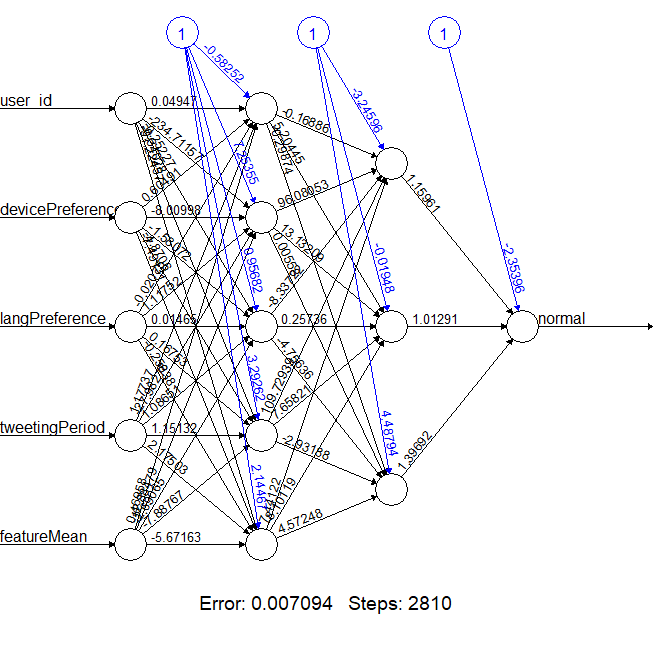
\includegraphics[scale=0.4]{sample_ann}
  \caption{Preview of ANN as created by R.}
\end{figure}

% \begin{figure}[h!]
%   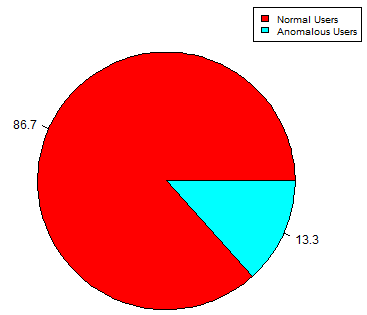
\includegraphics[scale=0.6]{pieChart1}
%   \caption{ Normal vs Anomalous Users.}
% \end{figure}

\newpage
\section{Conclusion and Futurework}

In this paper, we proposed an approach to identify Compromised account and detect Social Bots on the basis of behavioural features. Once the behaviour tends to change of what is considered to be normal, we flag the account as anamalous and the OSN admin can take necessary actions against the same. This work can be further extended for identifying several OSN attacks such as Cyberbullying, Identity Cloning, Sybil Account Detection, Creepers Attacks, Clickjacking etc on Twitter. Further, this work can be extended to be deployed on a decentralized network where the data is not centralized at one location.

\begin{center}
\textbf{References}
\end{center}

\begin{enumerate}[label={[\arabic*]}]
 \item Yazan Boshmaf, Konstantin Beznosov, and Matei Ripeanu. Graphbased sybil detection in social and information systems. In Advances in Social Networks Analysis and Mining (ASONAM), 2013 IEEE/ACM International Conference on, IEEE, 2013. 
  \item  Md Sazzadur Rahman, Ting-Kai Huang, Harsha V Madhyastha, and Michalis Faloutsos. Efficient and scalable socware detection in online social networks. In USENIX Security Symposium, pages 663–678, 2012. 
  \item  Zhi Yang, Christo Wilson, Xiao Wang, Tingting
        Gao, Ben Y Zhao, and Yafei Dai. Uncovering social
        network sybils in the wild. ACM Transactions on
        Knowledge Discovery from Data (TKDD), 2014. 
 \item ] Md Sazzadur Rahman, Ting-Kai Huang, Harsha V. Madhyastha,
and Michalis Faloutsos. Frappe: Detecting malicious facebook
applications. In Proceedings of the 8th International Conference on
Emerging Networking Experiments and Technologies, CoNEXT ’12,
pages 313–324, New York, NY, USA, 2012. ACM.
\item S. Yardi, D. Romero, G. Schoenebeck, and D. Boyd.
Detecting spam in a twitter network. First Monday,
15(1), 2010.
\item K. Thomas, F. Li, C. Grier, and V. Paxson.
Consequences of connectivity: Characterizing
account hijacking on twitter. Proceedings of the
ACM Conference on Computer and
Communications Security, pages 489–500, 2014.
 \item Manuel Egele, Gianluca Stringhini, Christopher Kruegel, and Giovanni
Vigna, Compa- detecting compromised accounts on social
networks. In NDSS, 2013.
 \item Phil McKenna. The rise of cyberbullying. New
Scientist, 195(2613):26–27, 2007.
\item Zhi Yang, Christo Wilson, Xiao Wang, Tingting
Gao, Ben Y Zhao, and Yafei Dai. Uncovering social
network sybils in the wild. ACM Transactions on
Knowledge Discovery from Data (TKDD), 2014.
\item Bimal Viswanath, M Ahmad Bashir, Mark Crovella, Saikat Guha,
MSR India, Krishna P Gummadi, Balachander Krishnamurthy, and
Alan Mislove. Towards detecting anomalous user behavior in
online social networks. In Proceedings of the 23rd USENIX Security
Symposium (USENIX Security), 2014. 

\item  Naeimeh Laleh, Barbara Carminati and Elena Ferrari. Risk Assessment in Social Networks based on
User Anomalous Behaviours, IEEE Transactions on Dependable and Secure Computing, 2015.

\item Rodrigo Augusto Igawa, Alex Marino Gonçalves de Almeida, Bruno Bogaz Zarpelao, Sylvio Barbon Jr.
XI Brazilian Symposium on Information System, Goiania, GO, May 26-29, 2015.

\item E. Zangerle and G. Specht. ”sorry, i was hacked” a
classification of compromised twitter accounts.
Proceedings of the ACM Symposium on Applied
Computing, pages 587–593, 2014.
\item Onur Varol, Emilio Ferrara, Clayton A. Davis, Filippo Menczer, Alessandro Flammini, Online Human-Bot Interactions: Detection, Estimation, and Characterization.
\item Rodrigo Augusto Igawa, Alex Marino Gonçalves de Almeida, Bruno Bogaz Zarpelão, Sylvio Barbon Jr,
Recognition of Compromised Accounts on Twitter, XI Brazilian Symposium on Information System, Goiˆania, GO, May 26-29, 2015.
\item Meike Nauta, Detecting Hacked Twitter Accounts by Examining
Behavioural Change using Twitter Metadata, IEEE, 2017.
\item Ting-Kai Huang, Md Sazzadur Rahman, Harsha V
Madhyastha, Michalis Faloutsos, and Bruno Ribeiro. An
analysis of socware cascades in online social networks.
In Proceedings of the 22nd international conference on
World Wide Web, pages 619–630. International World
Wide Web Conferences Steering Committee, 2013.
\item Ralph Gross and Alessandro Acquisti. Information
revelation and privacy in online social networks. In
Proceedings of the 2005 ACM workshop on Privacy in
the electronic society, pages 71–80. ACM, 2005.
\item Michael Fire, Roy Goldschmidt, and Yuval Elovici.
Online social networks- threats and solutions. 2013.
\item Phil McKenna. The rise of cyberbullying. New
Scientist, 195(2613):26–27, 2007.

\item Leyla Bilge, Thorsten Strufe, Davide Balzarotti, and
Engin Kirda. All your contacts are belong to us
automated identity theft attacks on social networks. In
Proceedings of the 18th international conference on
World wide web, pages 551–560. ACM, 2009.
\item L. Ablon, M. C. Libicki, and A. A. Golay. Markets
for Cybercrime Tools and Stolen Data: Hackers’
Bazaar. RAND Corporation, Santa Monica, CA,
2014.
\item S.-A. Bahrainian and A. Dengel. Sentiment analysis
and summarization of twitter data. In Computational
Science and Engineering (CSE), 2013 IEEE 16th
International Conference on, pages 227–234. IEEE,
2013.
\item S. Y. Bhat and M. Abulaish. Community-based
features for identifying spammers in online social
networks. In Proceedings of the 2013 IEEE/ACM
International Conference on Advances in Social Networks Analysis and Mining, pages 100–107. ACM,
2013.
% \item C. Chen, J. Zhang, X. Chen, Y. Xiang, and
% W. Zhou. 6 million spam tweets: A large ground
% truth for timely twitter spam detection. IEEE
% International Conference on Communications,
% 2015-September:7065–7070, 2015.

\end{enumerate}


\end{document}